\section{Scala}
\subsection{Introduction}
Scala belongs to the group of programming languages that can be compiled into Java byte code and run on a Java virtual machine (JVM). The major part, which makes it different from well-known Java, is the combination of applying a functional approach with an object-oriented paradigm. Together with the fact that Scala is similar to Java and it uses object-oriented principles, it can ease up transition for programmers who are unfamiliar with the functional world.

\subsection{Static vs. dynamic typing}
Besides the functional fundamentals, Scala belongs to the family of statically typed languages. This family also includes languages like C, C++, Java, or Haskell. Therefore, every single statement in Scala has a type.\cite{Scala static} Statically typed languages validates the type during compile time and once you compile it, you can run the compiled program multiple times.

On the other hand, dynamic typing does all type checking during runtime, and everytime you want to run the program, it is compiled again. Examples of languages, which use dynamic typing, are Python, Ruby and PHP.

\subsection{Strong vs. weak typing}
Strongly typed languages enforce strict restrictions on intermixing values with different datatypes. Thanks to that, the behaviour is more predictable than it would be for weak typed language. Majority of strongly typed languages require explicit declaration of type for each variable. However for Scala that's not entirely true. It is strongly typed language, but it uses a system known as type inference - automatic type detection. That allows faster coding, thanks to the fact that we don’t have to worry about specifying type for every statement. 

\begin{figure}[h]
  \makebox[\textwidth]{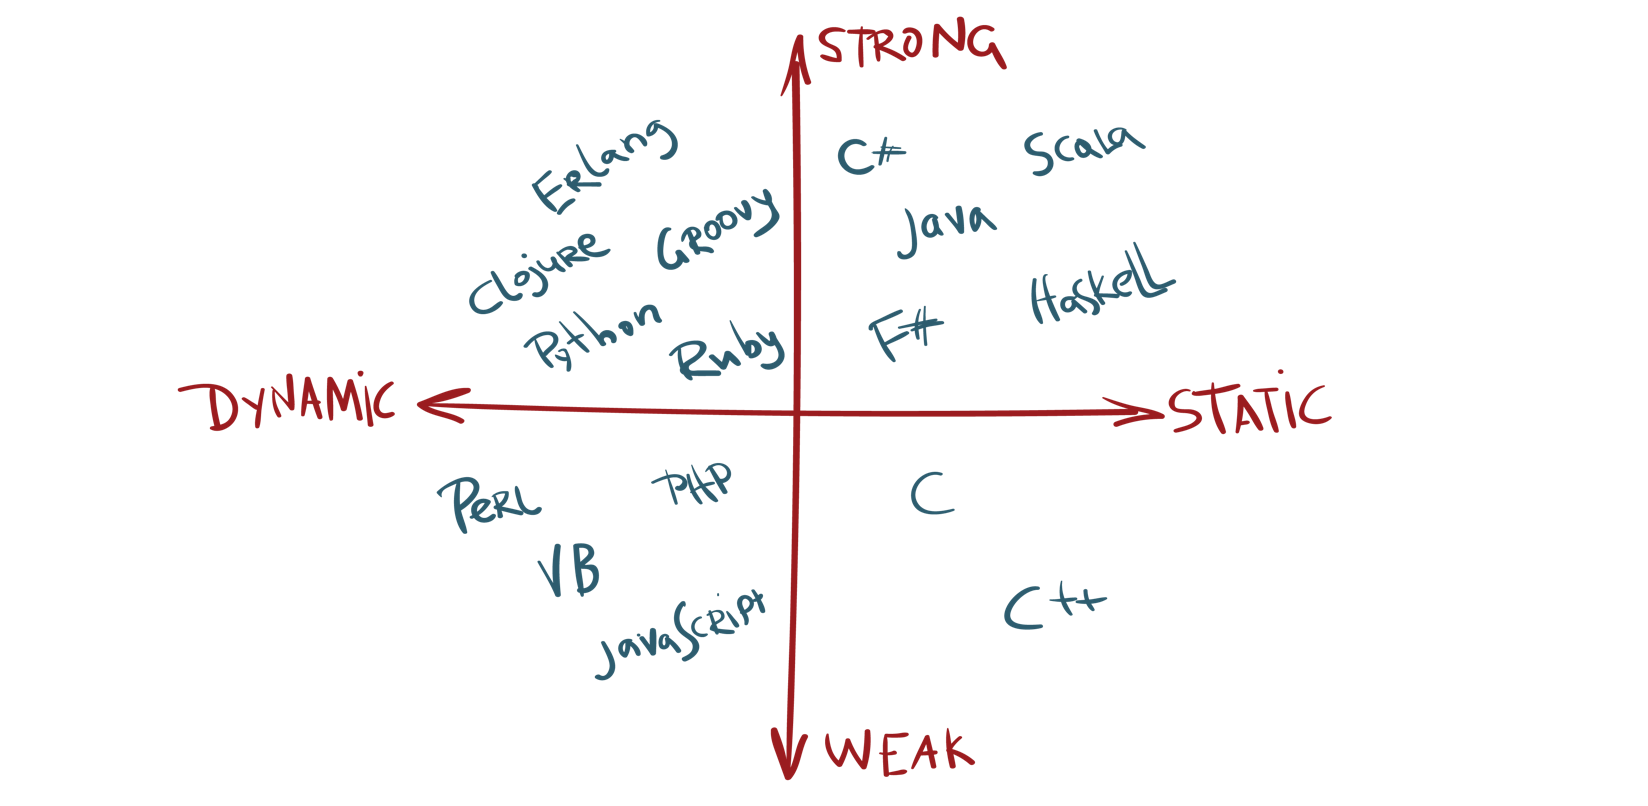
\includegraphics[width=\textwidth]{languages.png}}
  \caption {Languages divided into groups.\cite{Typing image}}
\end{figure}

